\chapter*{Le Base-ball multicolore}

On dispose de quatre bases de couleurs différentes, et deux joueurs associés à
chaque base. Le but du jeu est de déplacer les joueurs afin d'amener chaque
joueur sur la base correspondant à sa couleur. Il y a cependant trois
contraintes :

\begin{itemize}
\item les bases sont disposées en cercle, et un joueur ne peut se déplacer que
  vers les deux bases voisines (il ne peut pas traverser le terrain) ;
\item on ne peut déplacer qu'un joueur à la fois ;
\item chaque base a deux places, et un joueur ne peut se déplacer vers une base
  que si elle possède une place libre.
\end{itemize}

\begin{center}
  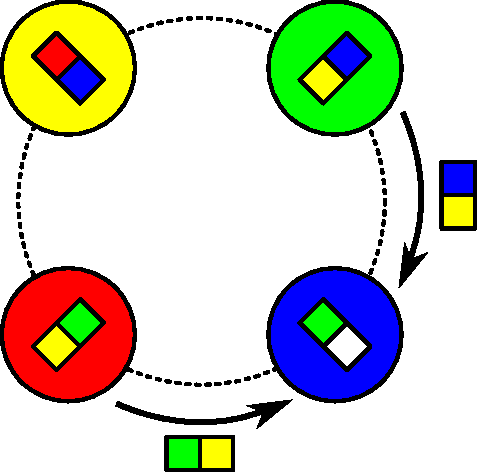
\includegraphics[width=0.3\linewidth]{algo1/baseball/baseball_coup.pdf}
  %\begin{tabular}{cc}
    %\etat{green}{blue}{red}{yellow}{white}{yellow}{green}{blue} &
    %\etat{red}{white}{green}{green}{blue}{blue}{yellow}{yellow} \\
    %État initial &
    %État final \\
  %\end{tabular}
\end{center}

\encart{Matériel}{
  \begin{itemize}
  \item Plusieurs équipes bien différenciables, chacune composée d'une base et
    de deux joueurs (des LEGO, des bouts de bois, des cailloux, du fil
    électrique de différentes couleurs, etc.)
  \item 4 équipes au minimum. On peut mettre des équipes ou des joueurs
    supplémentaires pour augmenter la difficulté.
  \end{itemize}
}

L'objectif de cette activité est d'\textbf{expliquer clairement} la méthode de
résolution du problème (algorithme), ainsi que le raisonnement qui a permis de
trouver cette méthode.

\newpage

\section*{Premier algorithme}

En suivant les règles du jeu, on observe que quelle que soit la disposition des
joueurs, 4 joueurs peuvent être déplacés vers la place vide : les deux de la
base de gauche, les deux de la base de droite. Notre algorithme sera donc une
méthode permettant de choisir à chaque étape quel coup jouer parmi ces 4
possibles.

\begin{itemize}
\item On ne s'autorise à tourner que dans un seul sens. Ainsi, le nombre de
  coups possibles descend de 4 à 2 (car 2 joueurs tourneraient à l'envers).
\item Parmi les 2 coups restants, on déplace le joueur qui a la plus grande
  distance à parcourir avant d'arriver à sa base (Si la distance est la même,
  c'est que les deux joueurs ont la même couleur - les deux coups sont alors
  équivalents).
\item Tant que tous les joueurs ne sont pas rentrés à leur base, on continue les
  déplacements.
\end{itemize}

% FIXME tikz ?
\begin{center}
  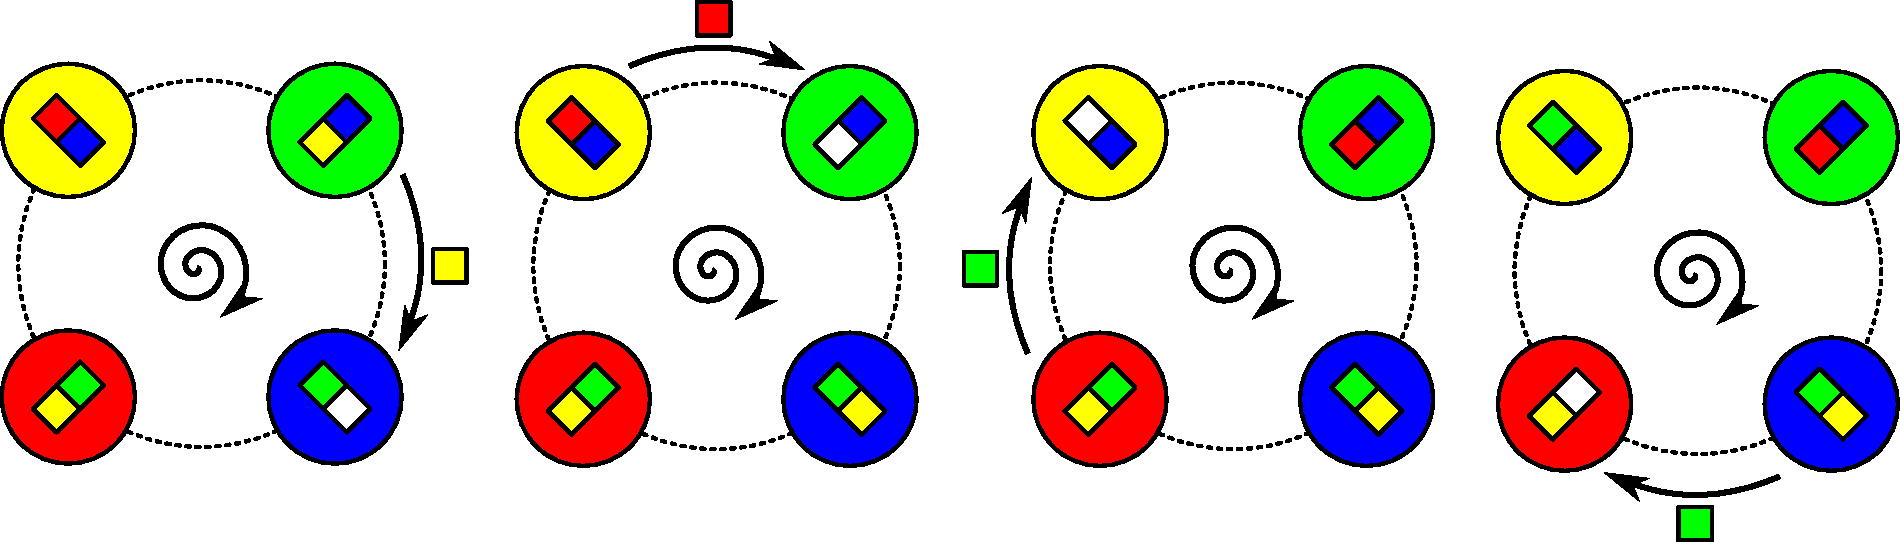
\includegraphics[width=\linewidth]{algo1/baseball/baseball_ex1.pdf}
\end{center}

Ici, nous n'avons représenté que les 4 premières étapes, mais l'algorithme
arrive à la solution en 15 étapes.

\subsection*{Regardons plus en détail{\ldots}}

À première vue, cet algorithme est attirant : il est assez simple et semble
relativement rapide --- 15 coups pour 4 bases et 7 joueurs --- ce n'est pas si
mal. Pourtant, il y a un problème : \textit{cet algorithme est faux}.

Pour s'en convaincre, il suffit de prendre le jeu dans son état résolu, et
d'intervertir deux joueurs. On observe alors que notre algorithme ramène le jeu
à son état initial sans atteindre la solution - notre algorithme boucle donc à
l'infini.

% FIXME tikz ?
\begin{center}
  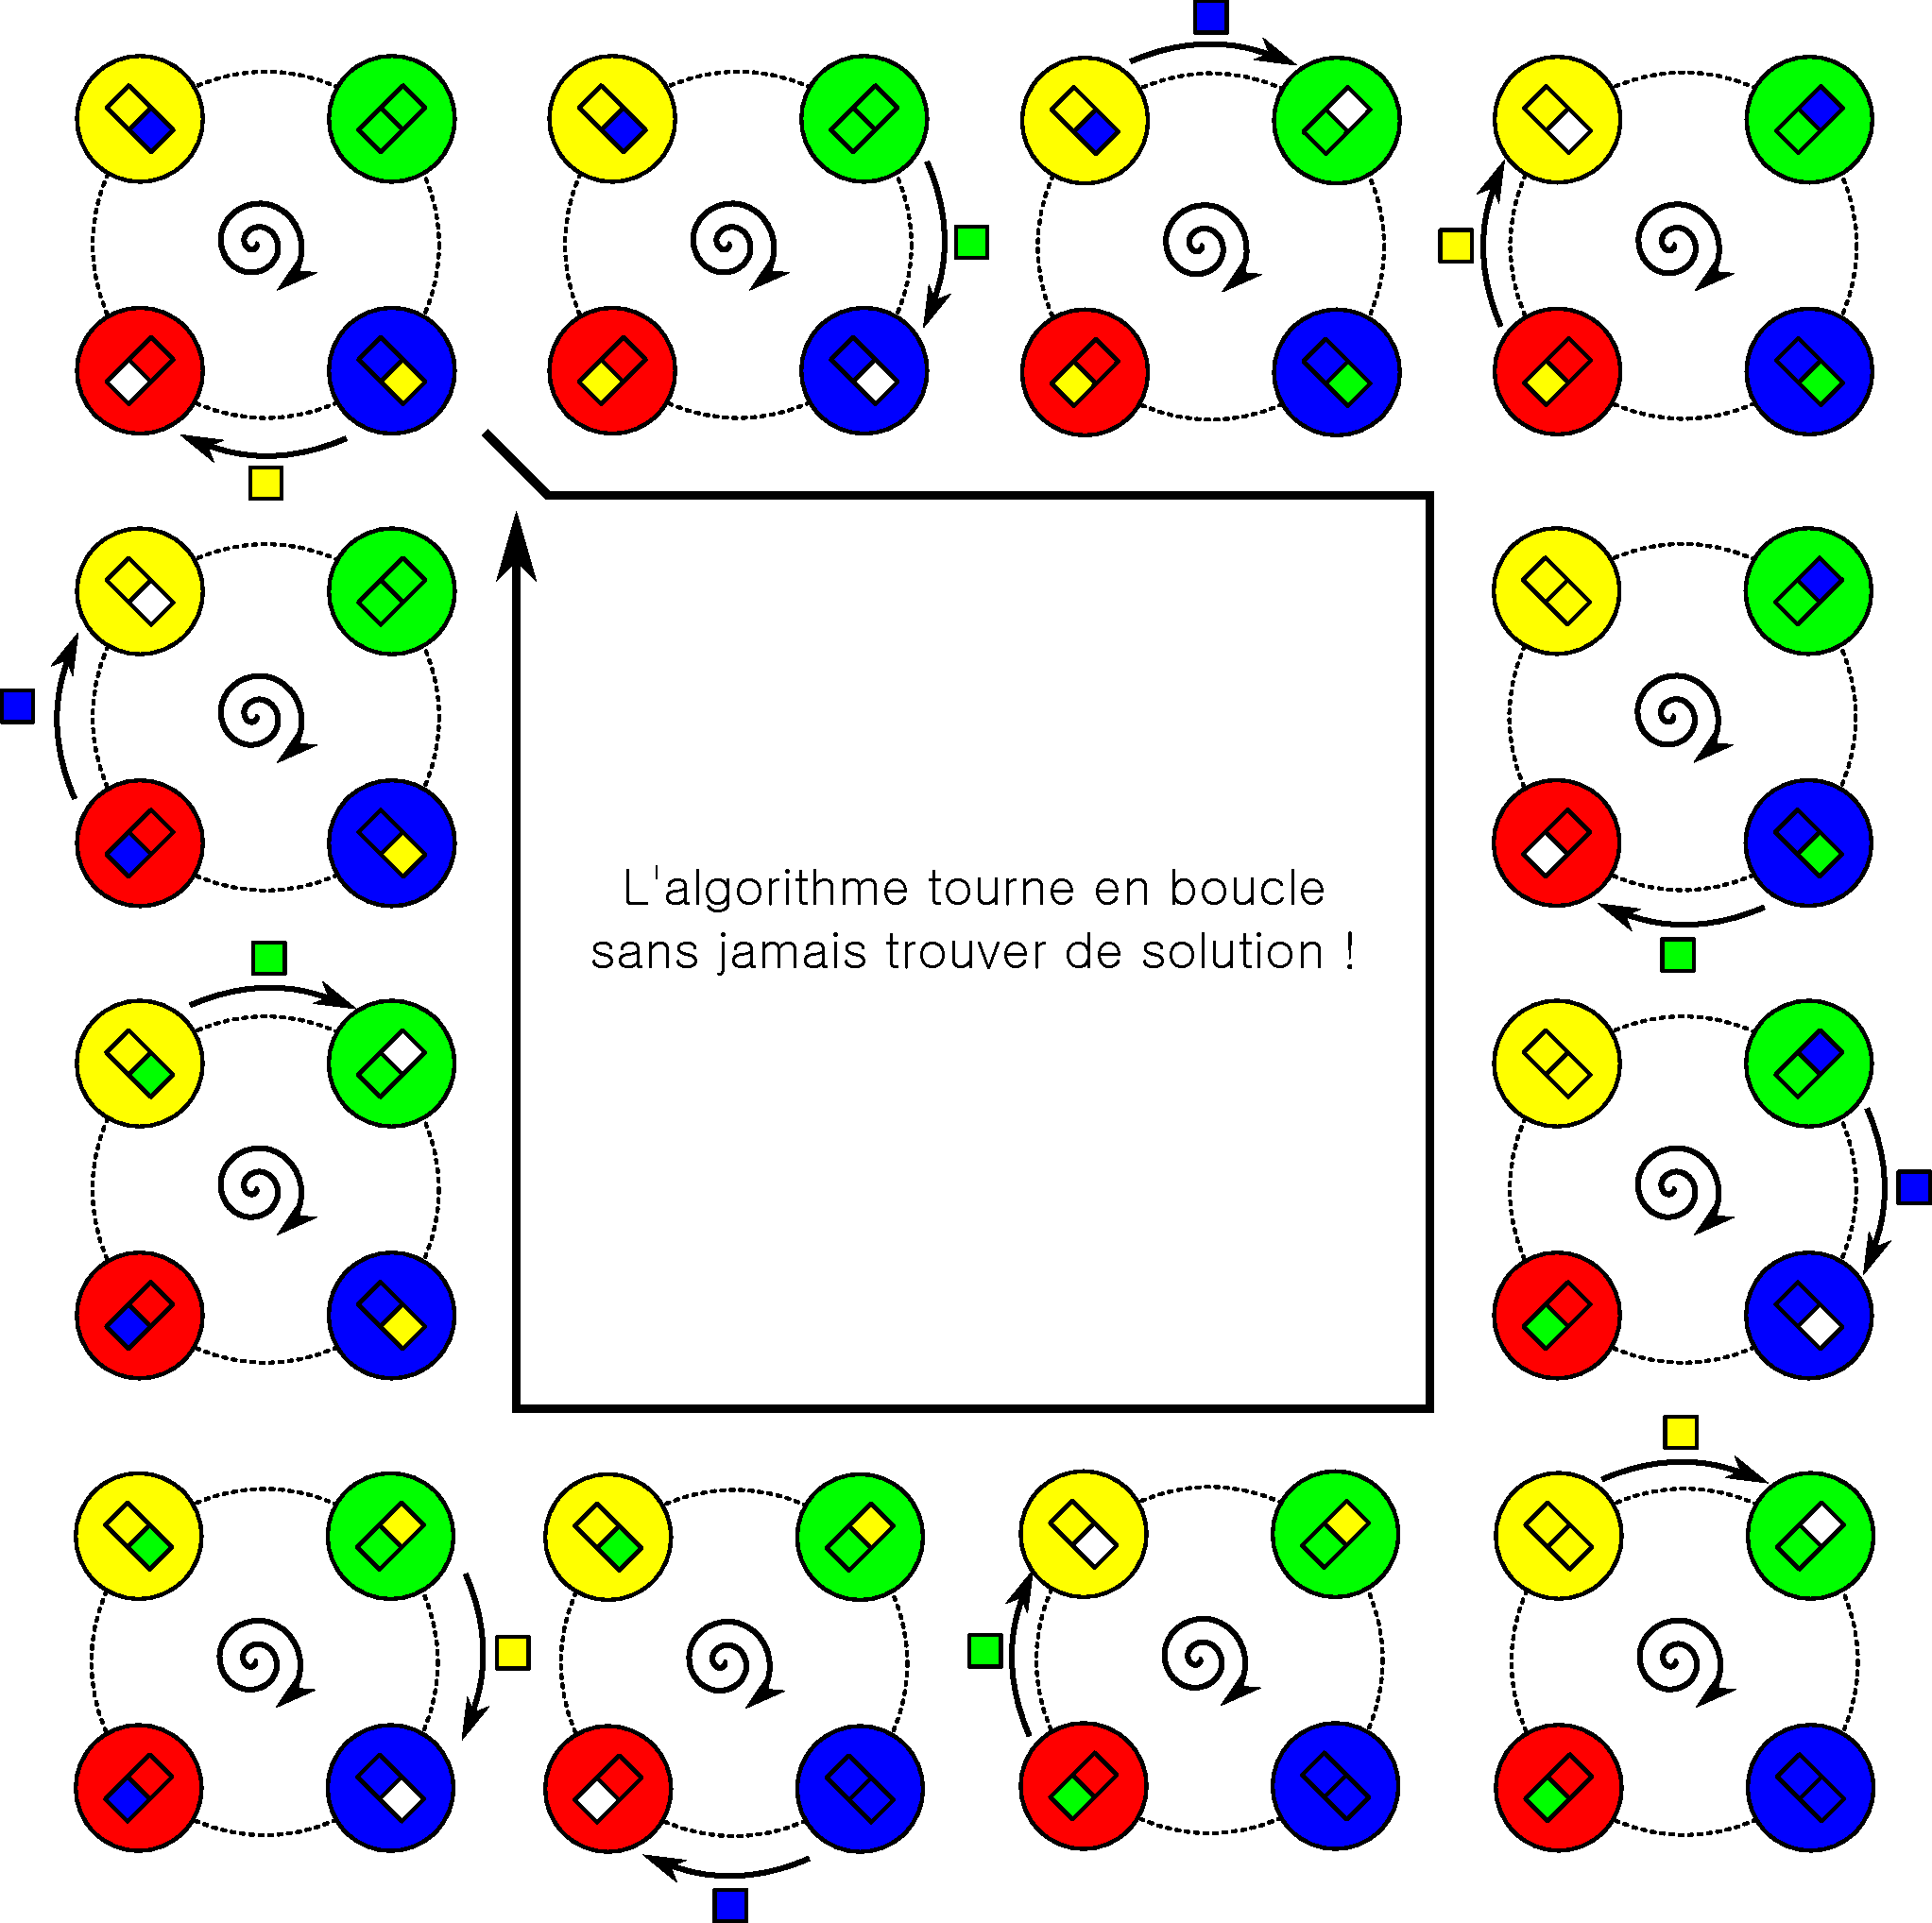
\includegraphics[width=\linewidth]{algo1/baseball/baseball_ex2.pdf}
\end{center}

\newpage

\section*{Deuxième algorithme}

Notre premier algorithme étant faux, réfléchissons à un autre algorithme. 

Commençons par \textit{apprendre de nos échecs}. Notre premier algorithme boucle
parfois à l'infini. Pour réparer cela, on pourrait s'interdire de faire un tour
complet en coupant le cercle. Pour ne pas se tromper, cela revient à disposer
les bases sur une ligne.

% FIXME tikz ?
\begin{center}
  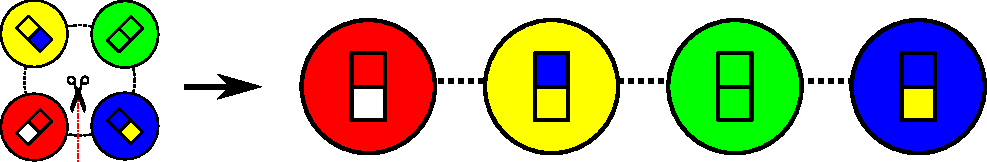
\includegraphics[width=\linewidth]{algo1/baseball/baseball_ligne.pdf}
\end{center}

Puis, \textit{apprenons de nos réussites}. Dans le problème du crêpier, on a
résolu le problème en réduisant progressivement sa taille : on place la première
crêpe, puis la deuxième etc. On s'est fixé des objectifs intermédiaires qui
décomposent le problème en étapes plus simples.

À partir de ces enseignements, on peut construire l'algorithme suivant :

% FIXME formulation complêtement merdique ! un ordi ne pourra pas comprendre ça ...
\begin{itemize}
\item On coupe le cercle de sorte que la base avec la place vide soit à
  l'extrémité droite.
\item On s'occupe des bases les unes après les autres, de gauche à droite.
\item Pour rapprocher un joueur de sa base, on déplace les joueurs des autres
  couleurs pour amener le trou à gauche du joueur à déplacer.
\item On répète l'opération jusqu'à ce que les deux joueurs soient revenus à
  leur base, et on n'y touche plus.
\end{itemize}

% FIXME tikz ? l'illustration est fausse, la base rouge devrait être à droite.
\begin{center}
  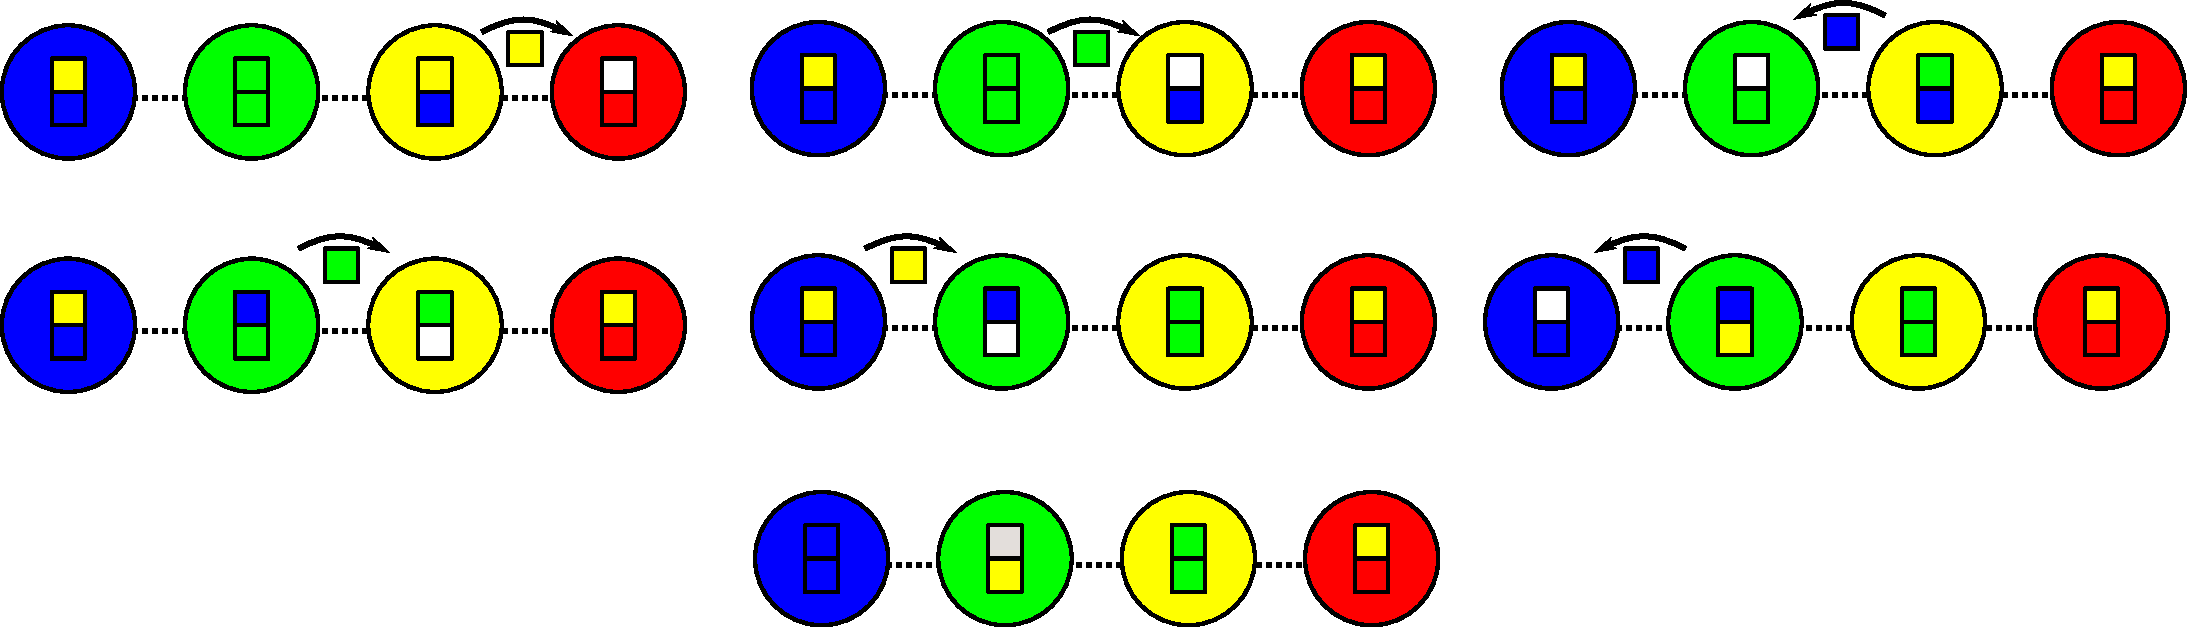
\includegraphics[width=\linewidth]{algo1/baseball/baseball_ex3.pdf}
\end{center}

On peut maintenant ignorer la première base, qui est déjà rentrée.

\section*{Correction d'algorithmes}

Notre deuxième algorithme est un peu plus complexe que le précédent, mais il est
correct --- une propriété très importante quand on écrit un algorithme. Mais
comment être sûr de la \textbf{correction} d'un algorithme ? Il existe plusieurs
approches :

\begin{description}
\item[Tester tous les cas.] On vérifie que l'algorithme trouve la solution pour
  tous les cas possibles. Mais ça ne marche que pour un problème de taille
  finie, et montrer de cette manière que notre algorithme est correct pour 4
  bases n'implique pas sa correction pour 5 bases.
\item[Écrire une preuve mathématique.] On peut prouver mathématiquement que cet
  algorithme fonctionne pour le cas général $m$ bases. Ce n'est pas trivial,
  mais les chercheurs en informatique en ont écrit des plus difficiles.
\item[Ça ressemble à un algorithme classique.] On peut observer une certaine
  ressemblance avec un algorithme déjà connu. Mais ça ne prouve rien, au
  fond{\ldots}
\end{description}

\subsection*{Les algorithmes classiques}

Les informaticiens apprennent par c\oe{}ur des algorithmes (abstraits) à
l'école. Face à un problème nouveau, un informaticien cherche généralement à le
ramener à un problème connu. Ce rapprochement se fait en trouvant des analogies
ou en décomposant le problème en plusieurs sous-problèmes connus.

Par exemple, quand des collègues informaticiens jouent au crêpier, ils demandent
avant tout si c'est \og une tour de Hanoï \fg, jeu bien connu des
informaticiens. Pour le base-ball multicolore, notre algorithme ressemble à un
\og tri à bulle \fg, autre algorithme bien connu. Mais cette ressemblance ne
suffit pas à prouver la correction de notre algorithme. Pour la prouver, il
faudrait démontrer que notre algorithme est un cas particulier du tri à bulle.
 
\subsection*{Les algorithmes de tri}

Les algorithmes de tri sont très classiques en informatique. D'une part, ils
permettent d'expliquer les grands principes aux élèves (\og diviser pour régner
\fg, récursivité, algorithmes gloutons {\ldots}). D'autre part, les ordinateurs
trient très souvent des données, car beaucoup de problèmes sont plus simples
après (trouver un livre est plus simple dans une bibliothèque rangée, par
exemple). \textit{Les musiciens font leurs gammes, les informaticiens débutants
  apprennent leurs algorithmes}.

%\subsection*{Le travail des chercheurs}

%Une partie du travail des chercheurs en informatique est d'améliorer les
% algorithmes connus, d'en inventer de nouveaux et de démontrer leur correction,
% d'en comparer les performances ...

\section*{Le coin de l'animateur}

L'objectif de cette activité est d'introduire la notion de correction
d'algorithme.

\begin{itemize}
\item Laissez les participants chercher un peu en les faisant verbaliser.
\item S'ils sont sur le point de trouver l'algo juste, introduisez très vite
  l'algo faux pour préserver un enchaînement logique~: \og oui, ok, mais je vais
  vous montrer une façon de faire rigolote. \fg
\item Quand l'algo juste est établi, et avant de parler de performance, on peut
  partir sur une variante :
  \begin{itemize}
  \item Chaque participant prend une couleur (une base placée au sol entre ses
    pieds)
  \item Chaque participant (sauf 1) prend un bonhomme dans chaque main
  \item À chaque étape, celui qui a une main libre prend un bonhomme dans la
    main d'un voisin
  \item (Attention, c'est fastidieux à 8 ou 9 couleurs, il vaut mieux faire deux
    rondes car l'algorithme semble $O(n^2)$)
  \end{itemize}
\item Expérimentalement, l'algorithme qui tourne converge très souvent vers la
  solution à 5 bases, mais converge souvent vers la boucle infinie quand il y a
  plus de couleurs. Ne tentez pas le diable ;)
\item Dans la disposition linéaire, il est plus simple de mettre la couleur avec
  un seul bonhomme à une extrémité, et commencer par remplir la maison de
  l'autre extrémité. Sinon, on se retrouve avec une maison remplie de un seul au
  milieu, et il faut comprendre que la solution passe par le stockage temporaire
  d'un pion de la maison d'à coté sur le trou.
\item Il serait intéressant de prouver effectivement la correction de
  l'algorithme linéaire, ainsi que de quantifier la probabilité de
  fonctionnement de l'algo qui tourne en fonction du nombre de maisons.
\end{itemize}


